\chapter{Cahier de Charges}

\section*{Introduction}%
\addcontentsline{toc}{section}{\numberline{}Introduction}%
Comme son nom ce chapitre a pour but de ressortir les différents éléments présents dans le cahier de charges d’un projet. Nous allons commencer par étudier la problématique dont fait face l’entreprise et de là nous allons ressortir les objectifs du projet. Ensuite nous aborderons les besoins et les contraintes. Puis nous allons terminer par la planification et l'estimation des couts.

\section{Contexte}
AMD est l'agent / distributeur exclusif au Cameroun de plusieurs categories de materiaux de maintenance industrielle. De ce fait la gestion commerciale est un element cle dans la survie economique de l'entreprise. AMD Sarl est une PME et comme la plupart des entreprises, pour leur aider dans la gestion de leurs activités au quotidien y compris la gestion commerciale, ils utilisent un outil de gestion commerciale en ligne, notamment l’ERP\footnote{Enterprise Resource Planning (Progiciel de Gestion Intégré en français)} Sage 100.
Cependant l'entreprise a souvent besoin d'optimiser le processus de fixation des prix de leurs produits ou encore savoir a quel moment avoir un certain produit en stock, ce qui pourrait nettement améliorer les ventes de l'entreprise. Ceci est rarement optimal. De ce fait ca devient plus difficile pour l'entreprise de fidéliser les clients ou encore acquérir des nouveaux clients. 

\section{Etude de l’existant}
Nous ne saurions débuter ce travail sans avoir une idée claire et précise sur l’existant quel qu’il soit. La première tâche a été de rencontrer les différentes personnes qui sont ou peuvent être impliquées dans les prises de décision et la gestion commerciale en général dans l’entreprise. 
\paragraph{}
Nous avons principalement travaillé avec le chef du département de l’approvisionnement, de la recherche et de l’innovation, M. Arnold KOGAING. Après quoi, nous avons réellement débuté le travail en menant différentes recherches. Cette méthodologie de travail nous a permis d’avoir une connaissance large de l’existant.

\subsection{La gestion commerciale à AMD}
AMD Sarl est une PME et comme la plupart des entreprises, pour leur aider dans la gestion de leurs activités au quotidien y compris la gestion commerciale, utilisent un outil de gestion commerciale en ligne, notamment l’ERP Sage 100.
\paragraph{}
Sage 100 est un logiciel qui propose d’accompagner les petites et moyennes entreprises dans la gestion de leurs ressources. De la gestion commerciale en passant par la comptabilité et les fonctionnalités de pilotage, Sage 100 s’impose comme un outil indispensable aux PME. Pour autant, la gestion des clients tout comme celle des achats et des fournisseurs ne sont pas en reste puisque Sage 100 propose une gestion puissante du cycle de vente du début de la chaîne jusqu’à sa fin.
\paragraph{}
Sage 100 est assez récent dans l’entreprise avec d’autres outils tels Gescom v14 et MS Excel utilisés pour gérer les processus de gestion commerciale. 

\subsubsection{Outils de gestion commerciale}
Le tableau \ref{tab:outilsdegescom} decrit un peu l'historique des outils des gestion commerciale utilisés par AMD.

\begin{table}[H]
    \centering
    \caption{Tableau des outils de gestion commerciale utilisés au fil du temps.}
    \begin{tabular}[t]{|p{3cm}|p{7cm}|p{5cm}|} 
        \hline
        \textbf{Outil} & \textbf{Description} & \textbf{Période} \\
        \hline\hline
        Sage 100 & ERP offrant de nombreuses fonctionnalitées & Moins de 10 mois d'utilisation \\
        \hline
        Gescom v14 & ERP, offrant moins de fonctionnalites que Sage 100 et les données sont moins descriptifs. Données pas aussi  fiables que celles de Sage 100  & Utilisation sur 3 années avant Sage 100 \\ 
        \hline
        Microsoft Excel & Tableur, permettant de concevoir de modèle de gestion assez complexes. Données encore moins fiables que celles de Gescom v14 & Utilisation sur 10 ans avant Gescom v14 \\ 
        \hline
        Traces papiers & Utilisation de papiers pour garder toute traces des transactions effectués par l’entreprise. & Dès la création de l’entreprise jusqu’à l’introduction de MS Excel. \\ 
        \hline\hline
    \end{tabular}
    \label{tab:outilsdegescom}
\end{table}%

\subsubsection{Prises de décisions en gestion commerciale}
Concernant de départements en entier, les décisions finales sont prises par le directeur général de l’entreprise après une ou plusieurs réunions avec les responsables dans le département en question et d’autres cadres. Ces réunions incluent souvent des brainstormings ou encore des analyses des chiffres. Il peut aussi arriver que le directeur se fie à son intuition pour prendre une décision. La figure \ref{fig:niveaudeladecision}, extraite d'un document en ligne\footnote{http://mmanagement.e-monsite.com/medias/files/les-decisions-et-parties-prenantes.pdf} intitulé \textit{"Décisions et le processus de décision"} montre les niveaux de décisions en entreprise.

\begin{figure}[H]
    \centering
    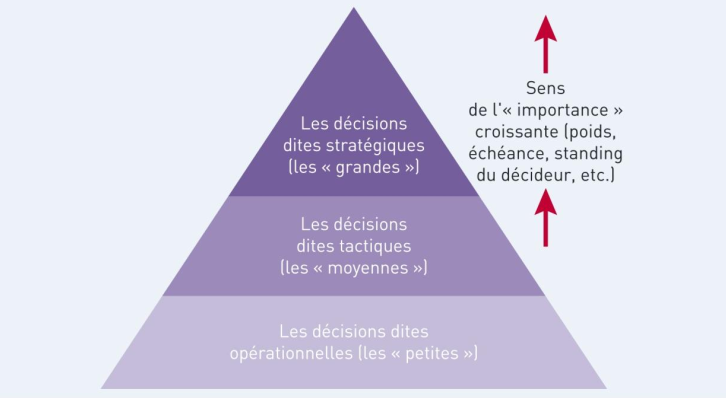
\includegraphics[width=\textwidth]{niveaudeladecision}
    \caption{Les niveaux de la décision}
    \label{fig:niveaudeladecision}
\end{figure}


Pour les décisions moins importantes, les chefs des différents départements ou services peuvent s’en charger suivant le même procédé que celui mentionné plus haut. En gros on recueille les points suivants dans la procédure de prise de décision.
\begin{itemize}
    \item Identifier la problématique à résoudre
    \item Identifier les différentes options possibles (brainstormings)
    \item Analyser les conséquences pour chaque option (analyses des chiffres)
    \item Définir l'option retenue (le directeur) et la mettre en oeuvre (les acteurs concernés)
\end{itemize}

\subsection{Critique de l’existant}
La critique de l'existant, appelée aussi bilan de l'existant, va nous aider à l'évaluation du système existant par rapport à la prise de décisions de gestion commerciale puisque c'est là que se pose nos problématiques. Ce diagnostic est établit dans le but de rechercher des solutions futures à des problèmes posés.
\paragraph{}
Le but de la critique de l'existant est d'établir un diagnostic précis sur les procédures utilisées, relever les anomalies, les qualités et les défauts du système existant.
\paragraph{}
Par ailleurs, deux aspects sont toujours dégagés lors de cette critique dont l'un est positif et l'autre négatif.Ces deux aspects méritent d'être soulevés étant donné que le besoin de la perfection sera toujours souhaité par les utilisateurs en vue de bon fonctionnement.

\subsubsection{Aspect(s) positifs}
Sous forme de liste on peut recenser les points positifs suivants dans le processus de prise de décisions.
\begin{itemize}
    \item Les opinions et analyses sont collectives
    \item Les chiffres (données) sont prises en considération dans le processus
    \item L'aspect \textit{"intuition"} est aussi considéré, ce qui garde notre nature humaine dans le processus.
\end{itemize}

\subsubsection{Aspect(s) négatifs}
Dans le processus de prise de décisions, l'analyse des chiffres intervient mais comme nous le savons tous, l'erreur est humaine. En ce faisant on peut rencontrer l'un des problèmes suivants, ce qui risque de mener à une mauvaise décision :

\begin{itemize}
    \item Mauvaise compréhension des chiffres
    \item Mauvaise correlation entre les différents sources ou rapports
    \item Ne pas analyser au delà des chiffres
    \item Focus sur la mauvaise métrique
\end{itemize}


\subsection{Les solutions concurrentes}
Nous avons vu plus haut les étapes du processus de prise de décisions. Il peut être reformulé de la façon suivante :
\begin{itemize}
    \item La phase de formulation ;
    \item La phase d’instruction ;
    \item La phase de choix ;
    \item La phase d’exécution.
\end{itemize}
\subsubsection{Techniques de prise de décisions}
Dans le processus mentionné plus haut c’est la troisième phase qui nous intéresse ici. On recense les techniques suivantes pour passer cette phase :
\begin{itemize}
    \item Se fier à l’intuition d’une ou plusieurs personnes
    \item Analyser les chiffres
    \item Utiliser un outil d’aide à la décision (Business Intelligence)
\end{itemize}

Nous avons vu plus haut quelques problèmes sur lesquels nous pouvons tomber en simplement analysant les chiffres sans outil d’aide. Aussi, l’intuition humaine peut s’avérer important dans certaines situations mais il est loin d’être suffisant pour prendre des décisions importantes. Nous pouvons ainsi conclure qu’un outil d’aide à la décision s’impose si nous voulons être optimal dans nos prises de décisions.

\subsubsection{Typologies des solutions de Business Intelligence}
\begin{itemize}
    \item \textbf{BI intégrée :} Il s’agit de solutions pouvant être intégrées à d’autres applications. Elle offrent des fonctionnalités analytiques et génèrent rapports et tableaux de bords ad hoc. Leur grande force réside dans leur capacité à s’intégrer à l’existant, y compris aux solutions de gestion d’éditeurs différents.
    \item \textbf{BI en libre service :} Il s’agit de solutions orientées utilisateur final : il n’a pas à se soucier du traitement en amont des données. Par le biais d’une interface conviviale, il peut librement explorer les données disponibles via des tableaux de bords personnalisables. On qualifie parfois ces solutions d’auto-suffisantes car elles accèdent à différentes sources de données pour en extraire des informations pertinentes sans le concours d’un service informatique dédié.
    \item \textbf{La DataViz :} Il s’agit de la data visualisation (visualisation de données) une fonction essentielle dans le traitement graphique des données traitées par la BI. Il s’agit de rendre intelligibles les informations traitées sous formes de graphes, tableaux et autres histogrammes. L’utilisateur final peut à loisir opter pour la visualisation qui correspond au traitement attendu des données. Contrairement à d’autres solutions, les applications de DataViz ne se connectent pas à des entrepôts de données non-structurées mais utilisent des bases de données déjà établies et/ou les données issues d’applications métiers. Il s’agit de fournir des indicateurs précis en temps réel afin de saisir un instantané opérationnel. La plupart du temps les tableaux de bord offrent une interface qui permet de les modifier par simple glisser-déposer.
    \item \textbf{Plate-forme de Business Intelligence : } Il s’agit d’outils complets de traitement des données structurées et non-structurées. Ils exploitent ces dernières afin d’en tirer une analyse pertinente, traduite elle aussi sous forme graphique. Ce type de solutions nécessite souvent un travail de développement et des spécialistes au sein d’un service informatique qui géreront le traitement des données en amont de l’utilisateur métier. Ce dernier peut alors se consacrer pleinement à l’analyse métier.
\end{itemize}
Nous avons plusieurs sources de données de différents types, nous voulons pouvoir faires des analyses et enfin visualiser ces données. Après cette étude nous sommes ressortis avec le tableau \ref{tab:comparatiftypebi} comparant les différents types de BI. Ceci nous guidera dans notre choix du type de solution à adopter.

\begin{table}[H]
    \centering
    \caption{Tableau comparatif des types de Business Intelligence.}
    \begin{tabular}[t]{|p{6cm}|p{3cm}|p{3cm}|p{3cm}|} 
        \hline
        \textbf{Typologie} & \textbf{Agrégation} & \textbf{Analyse} & \textbf{Visualisation} \\
        \hline\hline
        BI intégrée & Non & Non & \textbf{Oui} \\
        \hline
        BI en libre service & Non & Non & \textbf{Oui} \\
        \hline
        La DataViz & Non & \textbf{Oui} & \textbf{Oui} \\
        \hline
        Plate-forme de Business Intelligence & \textbf{Oui} & \textbf{Oui} & \textbf{Oui} \\
        \hline\hline
    \end{tabular}
    \label{tab:comparatiftypebi}
\end{table}%



\section{Problématique}
\subsection{Démarche d’analyse du problème}
Pour mieux analyser notre problème, on a résolu à utiliser la méthode des 5M. Aussi appelé diagramme de causes/effets" ou "en arêtes de poisson", l'outil créé par Mr Ishikawa fait partie de ceux à posséder dans sa trousse à outils spéciale "résolution des problèmes". Rappelant le squelette d'un poisson, cet outil visuel a pour finalité de lister les causes qui ont une influence sur un effet (une situation), de les classer, de les hiérarchiser. Très utilisé par les qualiticiens, le diagramme d'Ishikawa est en fait applicable à l'ensemble des métiers de l'entreprise.
\paragraph{}
Les étapes principales dans l’utilisation de cette méthode sont les suivants :
\begin{itemize}
    \item \textbf{Qualifiez l'effet :} Il s'agit couramment du problème que vous cherchez à résoudre. Dans notre contexte on peut identifier les effets suivants :
    \begin{itemize}
        \item La diffculté à fixer un prix pouvant generer un gain maximal à un moment précis
        \item Savoir a quel moment avoir un produit en particulier en stock et la quantité pour éviter des clients insatisfaits.
    \end{itemize}
    \item \textbf{Dressez un inventaire des causes possibles }: Il s’agit de lister les causes qui ont une influence sur le problème. Dans notre contexte on peut constater que l'entreprise possède des données généres par ses systèmes de gestion qui ne sont pas exploitées. De ce fait il ya un maque d'outils pouvant aider à faire des décisions.
    \item \textbf{Classez les causes par familles :} Ici intervient les 5M qui sont fréquemment utilisés pour cette tâche : Main d’œuvre, matière, matériels, méthodes, milieu. Dans notre cas on a une seule catégorie qui est la méthode d'utilisation de nos données.
    \item \textbf{Evaluez les branches/racines qui ont le plus d'impact.}
\end{itemize}

Le diagramme Ishikawa dans la figure \ref{fig:ishikawa} nous montre l'origine des problématiques dont fait face l'entreprise.
\begin{figure}[H]
    \centering
    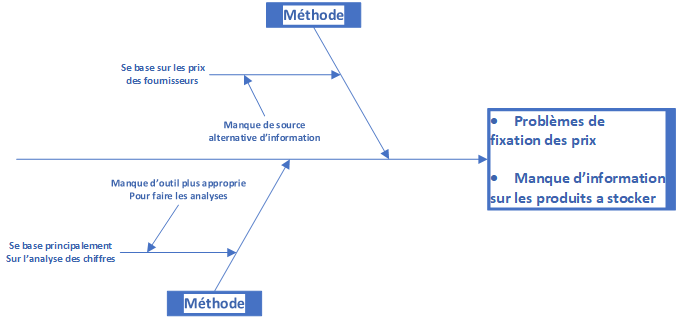
\includegraphics[width=\textwidth]{ishikawa}
    \caption{Diagramme Ishikawa analysant nos problématiques}
    \label{fig:ishikawa}
\end{figure}


\subsection{Identification de la problématique}
L’entreprise possède une quantité énorme d’informations non exploités, qui peuvent non seulement optimiser la prise de décisions par les décideurs mais aussi faciliter le travail des employés, augmentant ainsi la productivité de celles-ci, si exploitée de la bonne façon. 

De ce fait on peut identifier les difficultés  suivantes dont fait face l'entreprise, aussi représentés dans la figure 
\begin{itemize}
    \item La difficulté à fixer le prix d'un produit pour avoir un revenue maximal sur celui ci dans période bien précise.
    \item La difficulté dans l'identification des produits à mettre en stock avec les quantités à une certaine période pour éviter d'avoir des clients qui commandent des produits qu'on ne peut pas fournir.
\end{itemize}
De là on peut formuler notre problématique : \textbf{Comment fixer le prix des produits selon les périodes et savoir quand c’est pertinent de les avoir en stock ?}  



\section{Objectifs}
Après avoir posé nos problèmes, nous pouvons à présent parler des objectifs de notre projet.

\subsection{Objectif général}
L’objectif général c’est de mettre sur pied une plateforme de Business Intelligence, de l’intégration des données jusqu’à la visualisation en passant par l’analyse pour aider à la décision dans l'entreprise. 

\subsection{Objectifs spécifiques}
La solution devra nous permettre de :
\begin{itemize}
    \item Intégrer des données provenant de diverses sources notamment, l’ERP Sage 100, Gescom v14 et des fichiers Excel.
    \item Faire des analyses multidimensionnelles sur nos données.
    \item Visualiser nos données en masse et en ad hoc.
\end{itemize}


\section{Intervenants du projet}
Ce projet nécessitera pour sa réalisation :
\begin{itemize}
    \item Un (01) maître d'ouvrage qui est l'entreprise cliente ;
    \item Un (01) maître d'oeuvre qui est l'analyste, concepteur et Développeur du système ;
    \item Trois (03) consultants afin de pouvoir initier, cadrer et contrôler les travaux effectués ;    
\end{itemize}

Ces ressources sont matérialisées dans le tableau suivant :
\begin{table}[H]
    \centering
    \caption{Présentation des Intervenants du projet.}
    \begin{tabular}[t]{|p{4cm}|p{7cm}|p{4cm}|}
        \hline
        \textbf{Qualité } & \textbf{Nom} & \textbf{Fonction} \\
        \hline\hline
        Maître d'ouvrage & AMD Sarl & Porteur des besoins\\
        \hline
        Maître d'oeuvre & M. FOKOU DIFFO KANG Joel & Porteur du projet \\
        \hline
        Superviseur & Pr. AZEBAZE Anatole & Superviseur\\
        \hline
        Encadreur & M. TSAFACK Cédrique & Encadreur\\
        \hline
        Encadreur & M. DJATIO Christian & Encadreur\\
        \hline\hline
    \end{tabular}
    \label{tab:resmat}
\end{table}%



\section{Planification du projet}
Nous avons pu diviser notre projet en des grandes phases que nous allons représenter sur un diagramme de Gantt. Ces phases sont les suivantes : 
\begin{itemize}
    \item Identification du problème ;
    \item Etude de l’existant ;
    \item Analyse du projet
    \begin{itemize}
        \item Analyse fonctionnelle ;
        \item Analyse des couts ;
    \end{itemize}
    \item Etablissement du Cahier de Charges ;
    \item Conception du système ;
    \item Implémentation du système ;
    \item Test ;
    \item Installation.
\end{itemize}

La figure \ref{fig:gantt} représente le diagramme de Gantt du projet.


\begin{figure}[H]
    \centering
    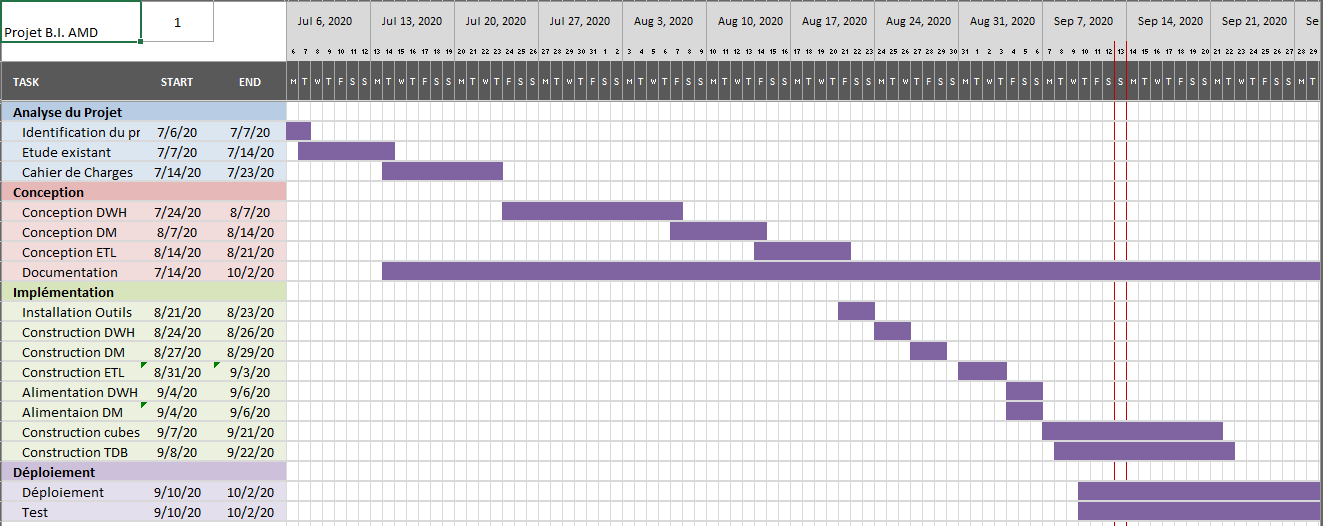
\includegraphics[width=\textwidth]{gantt}
    \caption{Diagramme de Gantt.}
    \label{fig:gantt}
\end{figure}


\section{Fonctionnalités attendus}
De façon générale le projet a deux fonctionnalités majeures. 
\begin{itemize}
    \item \textbf{Aide a la fixation des prix des produits par période définie}
    \item \textbf{Donner des indices pour savoir quand se ravitailler pour un produit}
\end{itemize}


\section{Besoins}
\subsection{Besoins Fonctionnels}
Pour notre système nous recensons les besoins fonctionnels suivants :
\begin{itemize}
    \item Suivre l'évolution des ventes par période
    \item Suivre les variations de prix 
    \item Suivre les commandes et les disponibilités par période
    \item Suivre les fréquences d'indisponibilité des produits.
\end{itemize}
\subsection{Besoins Non-Fonctionnels}
Hormis les besoins fonctionnels, nous voulons un système qui nous deonnera certains assurances tels quq :
\begin{itemize}
    \item \textbf{Sécurité : }Les données ne pourront pas etre accédés par des parties non autorisés.
    \item \textbf{Robustesse : }Le système doit être stable 
    \item \textbf{Disponibilité :}On doit pouvoir accéder au système en temps et en heure
    \item \textbf{Ergonomie : }Le système doit être facile et agréable a utiliser.
\end{itemize}
\section{Contraintes}
Ce projet fait face principalement a deux types de contraintes\begin{itemize}
    \item \textbf{Les contraintes techniques :} Ce projet a pour but d'aider à la décision, donc les techniques utilisées pour générer les résultats attendus doivent être précises.
    \item \textbf{Les contraintes temporelles :} Vu la date de de début du projet, le temps nécessaire pour compléter le projet est contraignant.
\end{itemize}


\section{Estimation des coûts}

\begin{table}[H]
    \centering
    \caption{Coût de ressources matérielles.}
    \begin{tabular}[t]{|p{3cm}|p{4cm}|p{2cm}|p{3cm}|p{3cm}|}
        \hline
        \textbf{Ressource} & \textbf{Caractéristiques} & \textbf{Quantité} & \textbf{Coût Unitaire} & \textbf{Coût Total}\\
        \hline\hline
        Ordinateur portable & Toshiba (i3-1.9GHz), Mémoire vive: 8GB & 01 & 200 000 FCFA & 200 000 FCFA\\
        \hline\hline
    \end{tabular}
    \label{tab:resmat}
\end{table}%

Dans le tableau \ref{tab:reshum} qui représente l'estimation des couts humaines pour le projet, on s'est basé sur la moyenne de salaires d'un developpeur de Business Intelligence au Cameroun pour estimer le prix d'une journée de travail de celui ci. Ceci nous a mené a la somme de \textbf{20 000 FCFA} par journée de travail. Et en se basant sur la méthode ascendante d'estimation des coûts on obtient le suivant.

\begin{table}[H]
    \centering
    \caption{Coûts des ressources humaines.}
    \begin{tabular}[t]{|p{2cm}|p{1.5cm}|p{3cm}|p{1.5cm}|p{3cm}|p{3cm}|} 
        \hline
        \textbf{Ressource} & \textbf{Nombre} & \textbf{Nom} & \textbf{Durée (jours)} & \textbf{Coût Unitaire} & \textbf{Coût Total}\\
        \hline\hline
        Analyste-Concepteur & 01 & FOKOU DIFFO KANG Joel & 34 & 20 000 FCFA & 680 000 FCFA\\
        \hline
        Développeur B.I. & 01 & FOKOU DIFFO KANG Joel & 31 & 20 000 FCFA & 620 000 FCFA\\
        \hline
        \textbf{Total} & \multicolumn{5}{c}{1 300 000 FCFA} \\
        \hline\hline
    \end{tabular}
    \label{tab:reshum}
\end{table}%


\begin{table}[H]
    \centering
    \caption{Coût total de développement.}
    \begin{tabular}[t]{|p{7cm}|p{8cm}|} 
        \hline
        \textbf{Ressource} & \textbf{Coût} \\
        \hline\hline
        Ressources Matérielles & 200 000 FCFA \\
        \hline
        Ressources Humaines & 1 300 000 FCFA \\
        \hline
        \textbf{Coût Total de développement} & \textbf{1 500 000 FCFA} \\
        \hline\hline
    \end{tabular}
    \label{tab:couttotal}
\end{table}%



\section*{Conclusion}%
\addcontentsline{toc}{section}{\numberline{}Conclusion}% 
Dans ce chapitre il était question de ressortir les éléments du cahier de charges et présenter les besoins. Nous avons terminé avec une planification et une estimation des couts du projet.